\documentclass[document.tex]{subfiles} 
\begin{document}
\section{Полученные результаты}
Практические результаты показали, что разработанный программно-аппа\-ратный комп\-лекс функционирует согласно заложенному алгоритму. Фотографии реализованного стенда приве\-дены на
рисунке~\ref{fig:stand} и в порядке очередности (слева-направо, сверху-вниз) иллюстриру\-ют следующие состояния программно-аппа\-ратного комплекса:
\begin{itemize}
  \item Выключен. Замеров инклинометром и вывода результатов не производится.
  \item Включен. Горизонтальное положение после встряски. Прямоугольник на дисплее сжат к центру, горит зеленый светодиод (встряска).
  \item Включен. Повернут на угол больше 30 градусов по X и Y. Прямоугольник растянут по X и по Y довольно сильно. Горит оранжевый светодиод (превышение отклонения
  уровня больше, чем на 30 градусов).
  \item Включен. Повернут на угол больше 30 градусов по X. Прямоугольник растянут по X довольно сильно, по Y меньше. Горит оранжевый светодиод (превышение отклонения
  уровня больше, чем на 30 градусов).
\end{itemize}
\begin{figure}[h]
\centering
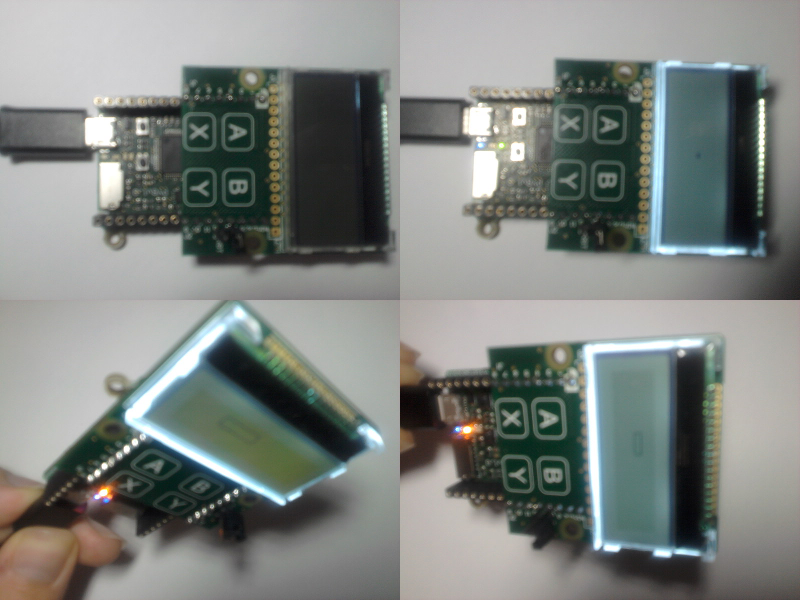
\includegraphics[width=0.9\linewidth,keepaspectratio]{stand}
\caption{Фотография стенда программно-аппаратного комплекса электронного уровня}
\label{fig:stand}
\end{figure}

\end{document}
